\begin{figure}[htbp]
\centering
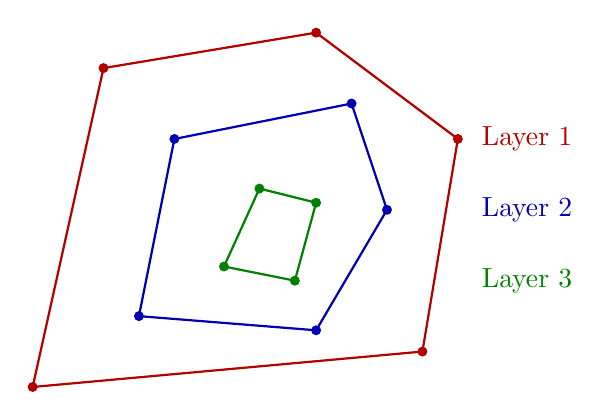
\begin{tikzpicture}[scale=0.9]
  \draw[thick,red!70!black] (-3,-2)--(-2,2.5)--(1,3)--(3,1.5)--(2.5,-1.5)--cycle;
  \node[red!70!black,right] at (3.2,1.5) {Layer 1};
  \draw[thick,blue!70!black] (-1.5,-1)--(-1,1.5)--(1.5,2)--(2,0.5)--(1,-1.2)--cycle;
  \node[blue!70!black,right] at (3.2,0.5) {Layer 2};
  \draw[thick,green!50!black] (-0.3,-0.3)--(0.2,0.8)--(1,0.6)--(0.7,-0.5)--cycle;
  \node[green!50!black,right] at (3.2,-0.5) {Layer 3};
  \foreach \p in {(-3,-2),(-2,2.5),(1,3),(3,1.5),(2.5,-1.5)} {\fill[red!70!black] \p circle (2pt);}
  \foreach \p in {(-1.5,-1),(-1,1.5),(1.5,2),(2,0.5),(1,-1.2)} {\fill[blue!70!black] \p circle (2pt);}
  \foreach \p in {(-0.3,-0.3),(0.2,0.8),(1,0.6),(0.7,-0.5)} {\fill[green!50!black] \p circle (2pt);}
\end{tikzpicture}
\caption{Convex hull peeling (onion peeling): successive convex hulls are removed, producing nested layers.}
\label{fig:onion_peeling}
\end{figure}
